\begin{tikzpicture}[]

    \pgfplotsset{
        % either use a `compat' level below or equal to 1.10, or change
        % `arc' coordinates (as done here)
        compat=1.10,
    }

\def\Wa{4}%
\def\Wb{2}%
\def\Wc{1}%

\begin{axis}[
	name=sinc1,
	y=1cm,
	x=0.4cm,
	 clip=false,
	 xmin=-9,xmax=9,
	 xlabel= $t$,
	 ylabel={$x_1(t)$},
	 ymin=-0.5,ymax=2,
	 axis lines=middle,
     	%xtick={-5, -4, ..., 5},
	 %ytick={-1, 1},
	 xticklabels=\empty,
	 yticklabels=\empty,
    ticks=none,
	 every axis x label/.style={at={(ticklabel* cs:1.0)}, anchor=south,},
	every axis y label/.style={at={(ticklabel* cs:1.0)}, anchor=west,},
		enlargelimits=true,
 ]
	%\addplot+[red, smooth, mark=none] table [x={n}, y={xn}] {periodic_square_fs_samples_of_envilope_gen.dat};
	\addplot [red!70!black, thick, domain=-3*pi:3*pi, samples=200] plot{\Wa/pi*sin(deg(\Wa*x))/(pi*x)};
	\node at (axis cs:-0.5, \Wa/pi) [anchor=east] { $W_1/\pi$ };
	\draw [latex-]  (axis cs:pi/\Wa, 0) ++ (0, -0.1cm) -- ++(0, -0.3cm) node [anchor=north] {$\dfrac{\pi}{W_1}$};
	\draw [latex-]  (axis cs:-pi/\Wa, 0) ++ (0, -0.1cm) -- ++(0, -0.3cm) node [anchor=north] {$-\dfrac{\pi}{W_1}$};
\end{axis}

\begin{axis}[
	name=rect1,
	at=(sinc1.south east), anchor=left of south west, xshift=1cm,
	y=1cm,
	x=0.4cm,
	 clip=false,
	 xmin=-5.1,xmax=5.1,
	 xlabel= $\omega$,
	 ylabel={$X_1(j\omega)$},
	 ymin=-0.5,ymax=1.2,
	 axis lines=middle,
	 ytick = {1},
     yticklabel style={above left},
	 xtick = {-\Wa, \Wa},	
	 xticklabels = {$-W_1$, $W_1$},
	 every axis x label/.style={at={(ticklabel* cs:1.0)}, anchor=south,},
	every axis y label/.style={at={(ticklabel* cs:1.0)}, anchor=west,},	
		enlargelimits=true,
	]
	\addplot [red!70!black, thick] coordinates  {(-5,0) (-\Wa, 0) (-\Wa,1) (\Wa, 1) (\Wa, 0) (5, 0)};
\end{axis}



\begin{axis}[
	name=sinc2,
	at=(sinc1.south), anchor=north, yshift=-0.8cm,
	y=1cm,
	x=0.4cm,
	 clip=false,
	 xmin=-9,xmax=9,
	 xlabel= $t$,
	 ylabel={$x_2(t)$},
	 ymin=-0.5,ymax=0.8,
	 axis lines=middle,
     	%xtick={-5, -4, ..., 5},
	 %ytick={-1, 1},
	 xticklabels=\empty,
	 yticklabels=\empty,
    ticks=none,
	 every axis x label/.style={at={(ticklabel* cs:1.0)}, anchor=south,},
	every axis y label/.style={at={(ticklabel* cs:1.0)}, anchor=west,},
		enlargelimits=true,
 ]
	%\addplot+[red, smooth, mark=none] table [x={n}, y={xn}] {periodic_square_fs_samples_of_envilope_gen.dat};
	\addplot [red!70!black, thick, domain=-3*pi:3*pi, samples=200] plot{\Wb/pi*sin(deg(\Wb*x))/(pi*x)};
	\node at (axis cs:-0.5, \Wb/pi) [anchor=east] { $W_2/\pi$ };
	\draw [latex-]  (axis cs:pi/\Wb, 0) ++ (0, -0.1cm) -- ++(0, -0.3cm) node [anchor=north] {$\dfrac{\pi}{W_2}$};
	\draw [latex-]  (axis cs:-pi/\Wb, 0) ++ (0, -0.1cm) -- ++(0, -0.3cm) node [anchor=north] {$-\dfrac{\pi}{W_2}$};
\end{axis}

\begin{axis}[
	name=rect2,
	at=(sinc2.south east), anchor=left of south west, xshift=1cm,
	y=1cm,
	x=0.4cm,
	 clip=false,
	 xmin=-5.1,xmax=5.1,
	 xlabel= $\omega$,
	 ylabel={$X_2(j\omega)$},
	 ymin=-0.5,ymax=1.2,
	 axis lines=middle,
	 ytick = {1},
     yticklabel style={above left},
	 xtick = {-\Wb, \Wb},	
	 xticklabels = {$-W_2$, $W_2$},
	 every axis x label/.style={at={(ticklabel* cs:1.0)}, anchor=south,},
	every axis y label/.style={at={(ticklabel* cs:1.0)}, anchor=west,},	
		enlargelimits=true,
	]
	\addplot [red!70!black, thick] coordinates  {(-5,0) (-\Wb, 0) (-\Wb,1) (\Wb, 1) (\Wb, 0) (5, 0)};
\end{axis}


\begin{axis}[
	name=sinc3,
	at=(sinc2.south), anchor=north, yshift=-1.2cm,
	y=1cm,
	x=0.4cm,
	 clip=false,
	 xmin=-9,xmax=9,
	 xlabel= $t$,
	 ylabel={$x_3(t)$},
	 ymin=-0.5,ymax=0.5,
	 axis lines=middle,
     	%xtick={-5, -4, ..., 5},
	 %ytick={-1, 1},
	 xticklabels=\empty,
	 yticklabels=\empty,
    ticks=none,
	 every axis x label/.style={at={(ticklabel* cs:1.0)}, anchor=south,},
	every axis y label/.style={at={(ticklabel* cs:1.0)}, anchor=west,},
	enlargelimits=true,
 ]
	%\addplot+[red, smooth, mark=none] table [x={n}, y={xn}] {periodic_square_fs_samples_of_envilope_gen.dat};
	\addplot [red!70!black, thick, domain=-3*pi:3*pi, samples=200] plot{\Wc/pi*sin(deg(\Wc*x))/(pi*x)};
	\node at (axis cs:-0.5, \Wc/pi) [anchor=east] { $W_3/\pi$ };
	\draw [latex-]  (axis cs:pi/\Wc, 0) ++ (0, -0.1cm) -- ++(0, -0.3cm) node [anchor=north] {$\dfrac{\pi}{W_3}$};
	\draw [latex-]  (axis cs:-pi/\Wc, 0) ++ (0, -0.1cm) -- ++(0, -0.3cm) node [anchor=north] {$-\dfrac{\pi}{W_3}$};
\end{axis}

\begin{axis}[
	name=rect3,
	at=(sinc3.south east), anchor=left of south west, xshift=1cm,
	y=1cm,
	x=0.4cm,
	 clip=false,
	 xmin=-5.1,xmax=5.1,
	 xlabel= $\omega$,
	 ylabel={$X_3(j\omega)$},
	 ymin=-0.5,ymax=1.2,
	 axis lines=middle,
	 ytick = {1},
     yticklabel style={above left},
	 xtick = {-\Wc, \Wc},	
	 xticklabels = {$-W_3$, $W_3$},
	 every axis x label/.style={at={(ticklabel* cs:1.0)}, anchor=south,},
	every axis y label/.style={at={(ticklabel* cs:1.0)}, anchor=west,},	
		enlargelimits=true,
	]
	\addplot [red!70!black, thick] coordinates  {(-4,0) (-\Wc, 0) (-\Wc,1) (\Wc, 1) (\Wc, 0) (4, 0)};
\end{axis}

\end{tikzpicture} 